\documentclass[]{myarticle}

\usepackage{mlbasemath}
\usepackage{mlcomplessita}

\makeatletter
\DeclareRobustCommand{\rvdots}{%
  \vbox{
    \baselineskip4\p@\lineskiplimit\z@
    \kern-\p@
    \hbox{.}\hbox{.}\hbox{.}
  }}
\makeatother

\usepackage{pgfplots}
\pgfplotsset{compat=1.5}
\usetikzlibrary{shapes,arrows,positioning,automata}

\usepackage[backend=bibtex]{biblatex}
\bibliography{multicore}

\author{Gabriele Atria \and Michele Laurenti}

\begin{document}

\title{Primo homework}
\maketitle

\section{Algoritmo ideale}

Trovare una password a forza bruta, conoscendone solo l'hash, equivale a cercare una stringa di lunghezza non determinata su un alfabeto.
Chiamiamo $\Sigma$ l'alfabeto su cui \`e costruita la stringa, e $\xi = \abs{\Sigma}$ il numero di caratteri nell'alfabeto.
La password che cerchiamo \`e una parola di $\Sigma^{\star}$ (l'insieme di tutte le parole costruite sull'alfabeto $\Sigma$).

L'idea algoritmica \`e la seguente: si enumerano tutte le stringhe in ordine quasi lessicografico (ordinandole prima per lunghezza, poi lessicograficamente), e si controlla se ciascuna di queste \`e la password cercata.
Se $n$ \`e la lunghezza della password, questo approccio permette di trovarla controllando non pi\`u di $\sum_{i = 1}^{n} \xi^i \simeq \xi^n$ stringhe.

L'implementazione ideale \`e scegliere di creare un numero ``infinito'' di thread, assegnando a ciascuno una parola, e schedulare per primi i thread a cui \`e stata data una parola che viene prima nel nostro ordinamento.
Il programma termina nel momento in cui un thread trova la stringa corrispondente alla password.

Possiamo rappresentare l'esecuzione dell'algoritmo ideale con un DAG (diretto verso il basso), in cui ogni nodo rappresenta un thread, e un arco orientato $(a,b)$ rappresenta la relazione ``$a$ termina prima dell'inizio di $b$''.

Con un solo processore a disposizione l'algoritmo visita i nodi da quello corrispondente alla parola pi\`u piccola a quello della password.
Possiamo quindi pensare il DAG con un solo processore come un cammino (figura \ref{fig:dag_seq}).
Assumendo che controllare se una stringa corrisponde alla password cercata abbia costo costante\footnote{In realt\`a l'algoritmo di hash avr\`a probabilmente un costo in funzione di $l$, la lunghezza della stringa di cui viene calcolato l'hash.}, il \emph{work} (tempo di esecuzione sequenziale) \`e $\bigo{\xi^n}$.

\begin{figure}[h]
	\centering
	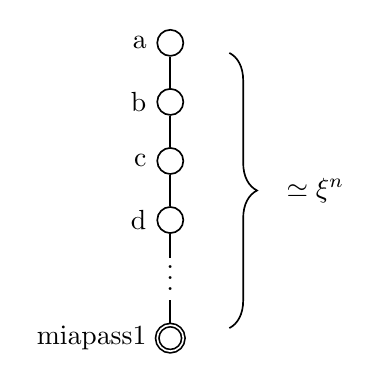
\begin{tikzpicture}[auto,semithick,node distance=.75cm]
		\node[circle,draw,label=left:a] (q0) {};
		\node[circle,draw,below of=q0,label=left:b] (q1) {};
		\node[circle,draw,below of=q1,label=left:c] (q2) {};
		\node[circle,draw,below of=q2,label=left:d] (q3) {};
		\node[below of=q3] (dots) {$\rvdots$};
		\node[circle,double,draw,below of=dots,label=left:miapass1] (qn) {};

		\node[right of=q0] (q0d) {};
		\node[right of=qn] (qnd) {};

		\draw (q0) -> (q1);
		\draw (q1) -> (q2);
		\draw (q2) -> (q3);
		\draw (q3) -> (dots);
		\draw (dots) -> (qn);
		\draw [decorate,decoration={brace,amplitude=10pt}]
		(q0d) -- (qnd) node [black,midway,xshift=0.6cm]
		{$\simeq \xi^{n}$};
	\end{tikzpicture}
	\caption{Il DAG di esecuzione dell'algoritmo sequenziale \`e un cammino lungo circa $\xi^n$.}
	\label{fig:dag_seq}
\end{figure}

Con $p$ processori, invece, il DAG di esecuzione di questo algoritmo possiamo pensarlo come un albero con $p$ figli, e ciascuno di questi figli \`e radice di un cammino lungo $\frac{\xi^n}{p}$ (figura \ref{fig:dag_par_p_proc}).

\begin{figure*}[th]
	\centering
	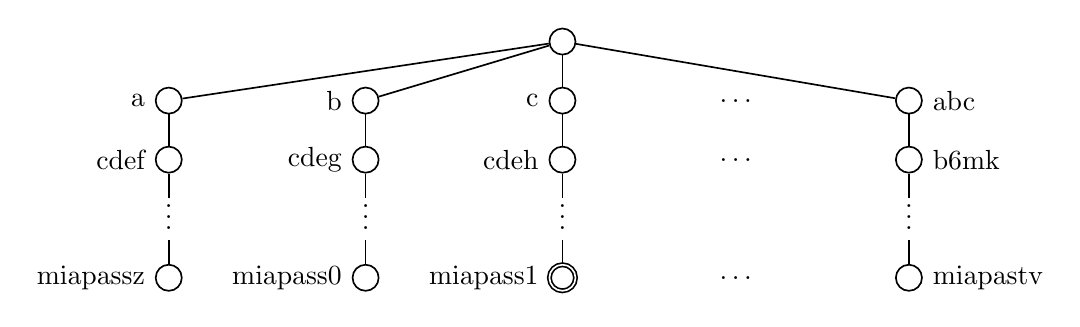
\begin{tikzpicture}[auto,semithick,node distance=.75cm]
		\node[circle,draw] (q0) {};
		\node[circle,draw,below of=q0,label=left:c] (q11) {};
		\node[circle,draw,node distance=2.5cm,left of=q11,label=left:b] (q21) {};
		\node[circle,draw,node distance=2.5cm,left of=q21,label=left:a] (q31) {};
		\node[right of=q11,node distance=2.2cm] (dots) {$\dots$};
		\node[circle,draw,node distance=2.2cm,right of=dots,label=right:abc] (q41) {};

		\node[circle,draw,below of=q31,label=left:cdef] (q32) {};
		\node[below of=q32] (3dots) {$\rvdots$};
		\node[circle,draw,below of=3dots,label=left:miapassz] (q3n) {};

		\node[circle,draw,below of=q21,label=left:cdeg] (q22) {};
		\node[below of=q22] (2dots) {$\rvdots$};
		\node[circle,draw,below of=2dots,label=left:miapass0] (q2n) {};

		\node[circle,draw,below of=q11,label=left:cdeh] (q12) {};
		\node[below of=q12] (1dots) {$\rvdots$};
		\node[circle,double,draw,below of=1dots,label=left:miapass1] (q1n) {};

		\node[circle,draw,below of=q41,label=right:b6mk] (q42) {};
		\node[below of=q42] (4dots) {$\rvdots$};
		\node[circle,draw,below of=4dots,label=right:miapastv] (q4n) {};

		\node[right of=q12,node distance=2.2cm] (dots1) {$\dots$};
		\node[right of=q1n,node distance=2.2cm] (dots2) {$\dots$};

		\draw (q0) -> (q11);
		\draw (q0) -> (q21);
		\draw (q0) -> (q31);
		\draw (q0) -> (q41);

		\draw (q11) -> (q12) -> (1dots) -> (q1n);
		\draw (q21) -> (q22) -> (2dots) -> (q2n);
		\draw (q31) -> (q32) -> (3dots) -> (q3n);
		\draw (q41) -> (q42) -> (4dots) -> (q4n);
	\end{tikzpicture}
	\caption{Il DAG di esecuzione dell'algoritmo parallelo \`e un albero che ha come figli della radice $p$ cammini lunghi ciascuno $\frac{\xi^{n}}{p}$.}
	\label{fig:dag_par_p_proc}
\end{figure*}

Quindi il tempo di esecuzione con $p$ processori \`e $\bigo{\frac{\xi^n}{p}}$.
Quindi lo speedup \`e lineare con $p$.

Lo \emph{span}, ossia il tempo di esecuzione con un numero infinito di processori, \`e $\bigo{1}$: viene creato un numero infinito di thread, ciascuno su un processore, e ciascun thread controlla una sola parola.

\subsection{Ottimizzazione dell'algoritmo ideale}

La situazione illustrata \`e ideale e non prende in considerazione l'impossibilit\`a pratica di creare infiniti thread.
L'implementazione che proponiamo dell'algoritmo cerca per\`o di avvicinarsi alla situazione ideale, in cui la sincronizzazione non ha costi:
\begin{enumerate}
	\item \label{itm:opt_word_set} Ciascun thread non lavora su una singola parola alla volta, ma su un insieme di parole di cardinalit\`a fissata, per ridurre il numero di thread totali.
		\`E quindi necessario trovare una partizione di $\Sigma^{\star}$ le cui classi abbiano tutte la stessa cardinalit\`a, e che sia possibile ordinare linearmente in modo che la classe $A$  preceda la classe $B$  se e solo se tutte le parole di $A$ precedono in ordine quasi lessicografico tutte le parole di $B$.
		Se le due propriet\`a sono verificate gli elementi dell'insieme quoziente saranno insiemi di parole verificabili nello stesso tempo e ordinabili ``rispettando'' l'ordine quasi lessicografico delle parole.

		La partizione che proponiamo inserisce in una classe tutte le parole lunghe $k$ che hanno in comune i primi $j$ caratteri, dove $j < k$.
		La differenza $k - j$ deve essere un'invariante per tutte le classi di questa partizione.
	\item Non creiamo un numero infinito di thread, che \`e solo una utile astrazione mentale, ma ne creiamo un numero $m$ che ripetono il lavoro finch\'e non trovano la password, e cerchiamo per quali valori di $m$ si ottiene lo speedup maggiore.
		In questa implementazione deve esistere un metodo che atomicamente ritorna una diversa stringa su $\Sigma$ in ordine quasi lessicografico, o meglio una classe di stringhe come da punto \ref{itm:opt_word_set}.
		Ciascun thread chiama questo metodo e controlla l'insieme di stringhe che riceve.
\end{enumerate}

\section{Implementazione}

\subsection{Implementazione ingenua}

La prima implementazione che proponiamo ricalca grossomodo l'algoritmo ideale.
Rappresentiamo ogni parola con una \code{String}, e attraverso due generatori di stringhe (\code{AllStringGenerator}, globale e sincronizzato, e \code{StringGenerator}, locale a ciascun thread) forniamo ai thread creati un ``inizio'' di parola e lasciamo loro il compito di concatenare questo inizio con tutte le possibili combinazioni di $n$ lettere.

La classe \code{AllStringGenerator} genera tutte le stringhe su un dato alfabeto.
La classe \code{StringGenerator} genera tutte le stringhe di una data lunghezza.

Le parole di lunghezza minore o uguale di $j$ (soglia che deve essere scelta opportunamente) vengono controllate in sequenziale all'inizio del programma.

Ciascun thread lavora su un insieme di parole e si sincronizza all'inizio del lavoro con la classe \code{Master} per ottenere l'insieme di password non ancora trovate.
Abbiamo scelto questa implementazione per evitare di dover mettere a disposizione dei thread un insieme di password sincronizzato (con lock di scrittura e di lettura), che avrebbe comportato l'acquisizione e il rilascio di un lock a ogni parola controllata.
Il draw-back di questa scelta \`e che i thread non termineranno il lavoro nel momento in cui l'ultima password viene trovata, ma se l'insieme di password su cui i thread lavorano \`e di dimensione ridotta l'attesa diviene trascurabile.

La struttura delle classi \`e rappresentata in figura \ref{fig:classi_progetto}.

\begin{figure*}[th]
	\centering
	\includegraphics[width=\textwidth]{homework1_classes.eps}
	\caption{Struttura delle classi del progetto.}
	\label{fig:classi_progetto}
\end{figure*}

Abbiamo scelto di parametrizzare, oltre al numero di thread, anche la dimensione dei blocchi di lavoro.
Cerchiamo di illustrare il motivo di questa scelta.

La dimensione dei blocchi di lavoro determina il numero di operazioni sincrone (e quindi sequenziali) che devono essere fatte (in particolare, \code{getPassowrds} e \code{getNextWord}).
Se $n$ \`e la lunghezza della password e $j$ la dimensione del blocco di lavoro, la percentuale di operazioni sincrone dipender\`a da $\frac{1}{36^j}$.

Come detto poco sopra la dimensione dei blocchi di lavoro comporta una ``coda'' di lavoro inutile dopo che \`e stata trovata l'ultima password.
L'impatto di questo lavoro inutile sull'esecuzione del programma dipende dal rapporto fra $j$ e $n$ (e non dal numero di processori).

Abbiamo quindi due fattori che limitano lo speedup del programma: per valori di $j$ vicini ad $n$ la ``coda'' dell'esecuzione avr\`a una durata paragonabile alla durata del resto del programma; se invece il rapporto fra $j$ ed $n$ \`e trascurabile, lo speedup (secondo Amdahl) \`e limitato dalla percentuale di operazioni sincrone, e dipende quindi da $36^{j}$.

\`E difficile quantificare precisamente il peso della coda e delle operazioni sincrone, ma quello che abbiamo cercato di illustrare \`e che la dimensione dei blocchi di lavoro deve essere una qualche funzione del numero di processori e della (supposta) lunghezza della password.
Nei test che abbiamo condotto questo non \`e visibile, poich\'e il numero di processori e la lunghezza delle password sono molto bassi.

\subsection{Piattaforma dei test}

I computer su cui abbiamo testato l'algoritmo sono:
\begin{itemize}
	\item un Raspberry Pi 2 Model B, con CPU ``900 MHz quad-core ARM Cortex-A7'' secondo wikipedia \cite{wikipi};
	\item un computer fisso con processore ``Intel Core i5 (650) 3.2 GhZ dual-core'', con hyperthreading (e possibilit\`a di disattivarlo);
	\item un iMac $27''$ ``11,1'' con processore ``Intel Core i7 (860) 2.8 GHz quad-core'', con hyperthreading.
\end{itemize}

Nei test condotti abbiamo fissato un tetto alla lunghezza della password e generato password casuali fino a questa lunghezza, assieme all'ultima password in ordine quasi lessicografico di quella lunghezza.
Con lunghezza 4, il programma deve cercare $n$ password di lunghezza minore o uguale a 4 e l'hash della password ``\code{9999}''.
Evitiamo quindi casi limite in cui le $n$ password generate sono tutte ``vicine'' e con un basso indice quasi lessicografico, costringendo il programma a provare (almeno) tutte le parole da ``\code{a}'' a ``\code{9999}''.

La lunghezza delle password \`e stata scelta da computer a computer, per arrivare a test della durata di qualche ora.

Nel calcolo dello speedup abbiamo considerato come tempo sequenziale il tempo di esecuzione dell'algoritmo con un solo thread.

\subsubsection{Risultati attesi}

Ci aspettiamo di vedere:
\begin{itemize}
	\item speedup lineare;
	\item speedup massimo quando il numero di thread \`e uguale al numero dei processori;
	\item buon load balancing.
\end{itemize}
I primi due risultati saranno evidenti dai tempi di esecuzione.

Il terzo riteniamo di poterlo dedurre da un eventuale speedup massimo e lineare con pochi thread: significherebbe che il lavoro \`e ben distribuito anche fra questi pochi thread, che riescono a sfruttare al meglio i processori a disposizione.
Inoltre l'algoritmo assegna blocchi di lavoro di uguale dimensione a ogni thread, e poich\'e il numero di questi blocchi (in una situazione reale) \`e molto maggiore del numero di processori ($36^{n-j}$ blocchi contro $p$ processori) ci aspettiamo che ogni thread lavori su circa $\frac{36^{n-j}}{p}$ blocchi di lavoro.

\subsubsection{Risultati ottenuti}

I risultati sul Raspberry Pi sono differenti con le due JVM utilizzate.
\begin{itemize}
	\item Con la JVM OpenJDK i tempi sono piuttosto lunghi, ma lo speedup \`e praticamente lineare.

	Oltre i 4 thread l'algoritmo ha crashato circa un quinto delle volte per un ``unhandled signal 11''.
	Un rapida ricerca su internet mostra che il segnale indica un segmentation fault.
	Stupiti, seguendo il consiglio di \cite{getrealjava}, cambiamo JVM.
	\item Con la JVM Oracle i tempi sono sensibilmente pi\`u corti, ma lo speedup si arresta intorno a 3.
	I grafici di utilizzo della CPU mostrano che non viene utilizzato pi\`u del 75\% dei 4 processori, il che spiega la limitazione dello speedup.
	Ipotizziamo che lo scarso utilizzo dei processori sia dovuto al garbage collector della JVM Oracle.
	Informazioni trovate su internet indicano che l'azione del garbage collector \`e una parte forzatamente sequenziale del codice, poich\'e ferma l'esecuzione di ogni thread.
	La prima implementazione dell'algoritmo usa un gran numero di oggetti immutabili (fra \code{String} e \code{BigInteger}), facendo lavorare molto il garbage collector.
\end{itemize}

Con l'i5 abbiamo avuto la possibilit\`a di testare l'algoritmo con e senza hyperthreading.
Con hyperthreading abilitato e aumentando il numero di thread lo speedup migliora leggermente, e supera il numero di core fisici, ma resta molto inferire al numero di core logici.
Ipotizziamo che l'hyperthreading porti a risultati migliori, anche se non ne conosciamo il funzionamento.

Con l'iMac i risultati sono tragici: usando 3 thread si raggiunge gi\`a lo speedup massimo, molto inferiore allo speedup lineare.
La causa potrebbe essere sempre il troppo lavoro del garbage collector.

\`E evidente che la prima implementazione \`e fortemente ottimizzabile: lo speedup non \`e assolutamente lineare come ci saremmo aspettati.
La seconda implementazione, con le ottimizzazioni descritte nel seguito, ci aspettiamo abbia un comportamento pi\`u vicino a quello dell'algoritmo ideale.

\subsection{Ottimizzazione del'implementazione}

Le ottimizzazioni che abbiamo implementato sono le seguenti:
\begin{itemize}
	\item rappresentiamo le parole con \code{byte[]}, invece di \code{String}.
	I vantaggi sono diversi: l'implementazione di md5 prende in input e d\`a in output \code{byte[]}, il che ci risparmia almeno due conversioni di tipo; non creiamo $\bigo{36^n}$ nuove stringhe (che sono tipi immutabili), ma possiamo riutilizzare lo stesso \code{byte[]}.
	\item vale un discorso simile sostituendo \code{int} a \code{BigInteger}: passiamo da un tipo immutabile a un tipo mutabile, per la gioia del garbage collector.
	\item la struttura dati che accoglie le password \`e un \code{TreeSet<byte[]>}, con associato un \code{Comparator<byte[],byte[]>}, che ci permette di effettuare operazioni di ricerca e rimozione in $\log(n)$ (dove $n$ \`e il numero di password).
	Per $n$ sufficientemente grandi \`e un vantaggio rispetto a una ricerca lineare su una struttura non ordinata: per ogni parola bisognerebbe controllare tutti gli $n$ hash, dato che la probabilit\`a di trovare una password \`e molto bassa.
	\item l'insieme di password, mantenuto dal \code{Master}, non viene copiato da \code{getPasswords}: il metodo ritorna (senza sincronizzazione) il riferimento all'insieme del master.
	Nel momento in cui viene trovata una password, il master si occupa (con sincronizzazione) di duplicare l'insieme di password, rimuovere la password trovata, e di cambiare il proprio riferimento.

	L'implementazione del metodo \code{foundPassword} non lascia l'insieme di password in uno stato intermedio e non corretto: per questo siamo portati a concludere che il metodo \code{getPasswords} non ritorner\`a mai un insieme di password in uno stato inconsistente.
\end{itemize}

\subsubsection{Risultati ottenuti}

I tempi di esecuzione sono diminuiti di un fattore compreso fra 4 e 8.

Con il Raspberry Pi lo speedup ora \`e poco sotto il lineare, anche con la JVM Oracle.
Non si sono verificati altri segmentation fault.

Con l'i5, senza hyperthreading, i tempi sono pi\`u corti rispetto alla prima implementazione, ma lo speedup \`e praticamente identico.
Con hyperthreading attivo lo speedup massimo che otteniamo \`e maggiore rispetto alla prima implementazione: si aggira intorno a 2.9, contro il 2.2 che avevamo in precedenza.
Il risultato ci sembra buono, considerato che i core fisici sono solo 2, anche se non \`e lineare nel numero di core logici.

Con l'iMac, gli effetti dell'hyperthreading sembrano essere positivi con la seconda implementazione: lo speedup \`e vicino al lineare (nel numero di core fisici), e supera il numero di core fisici arrivando a circa 5.
L'andamento non \`e comunque regolare.

\section{Conclusioni}

Dai risultati nascono alcune considerazioni:
\begin{itemize}
	\item con parole troppo corte lo speedup non \`e visibile.
	Ipotizziamo sia dovuto al rapporto fra parti sequenziali dell'algoritmo (principalmente inizializzazione e sincronizzazione) e parti parallele, che per password corte \`e pi\`u alto.
	\item lo speedup non \`e \emph{esattamente} lineare nel numero di processori.
	In accordo con la legge di Gustafson le parti sequenziali dell'algoritmo ``abbassano'' la pendenza della retta dello speedup, rendendolo quindi meno che lineare.
	Riteniamo che, per il ragionamento descritto nella sezione sull'implementazione dell'algoritmo, aumentando nel modo opportuno il numero di processori, la lunghezza della password e la dimensione dei blocchi di lavoro lo speedup si avviciner\`a ulteriormente allo speedup lineare.
	\item i grafici mostrano che la nostra previsione non era infondata: abbiamo ottenuto speedup massimo quando il numero di thread \`e uguale al numero di core (fisici senza hyperthreading, logici con hyperthreading).
\end{itemize}

Le considerazioni sono molto parziali: l'hyperthreading complica l'interpretazione dei risultati, e il numero di core fisici dei computer su cui abbiamo eseguito i test \`e basso.

\`E facile pensare un'implementazione distribuita dell'algoritmo, dopo le dovute considerazioni.
L'algoritmo non ha problemi di fiducia: nel momento in cui assegna un inseme di parole a un thread, assume che questo le controlli tutte.
Se eseguito su pi\`u computer l'algoritmo deve tenere traccia degli insiemi di parole che ha distribuito per assegnare a un nuovo \emph{worker} insiemi che restano ``orfani'' in caso di fallimenti.

Ci sono poi alcune ottimizzazioni che non abbiamo considerato, preferendo un'implementazione semplice che ci permettesse di concentrarci sull'analisi dell'algoritmo.
Una su tutte \`e quella di interrompere i thread nel momento in cui tutte le password sono state trovate, eliminando il problema della ``coda'' di esecuzione.

\subsection{Esecuzione dell'algoritmo}

Abbiamo creato un \code{Makefile} per la compilazione il programma.
Un modo possibile per eseguirlo \`e \code{java -cp ./bin homework\_seconda\_implementazione.Main [nome\_file].txt}.

Visti i risultati ottenuti, il \code{Main} indicato sopra esegue l'algoritmo con un numero di thread pari al numero di processori a disposizione, e con la dimensione dei blocchi di lavoro fissata a \code{2}, un numero magico che sembra comportarsi bene nei test condotti.

\renewcommand{\refname}{Riferimenti}

\printbibliography

\end{document}
